\section{Performance}
\sectiontoc

\tikzset {
    graph/.style = {
        mark=x,
        line width=1pt,
        line cap=round,
    },
}

\subsection{Theoretical Limits}
\begin{frame}{Theoretical Limits}
    \begin{quote}
        A well designed Lustre storage system can achieve
        90\% of underlining hardware bandwidth.

        \hspace*\fill{\scriptsize--- Zhiqi Tao, Sr. System Engineer, Intel \cite{10-intel}}
    \end{quote}

    \pause

    \textbf{Example}

    \begin{itemize}
        \item<+-> 160 OSS, 16 OST each, 2 TiB each
        \item<+-> $\rightarrow$ 2.5 PiB (Pebibyte) total storage
        \item<+-> each OST delivers 50 MiB/s
        \item<+-> $\rightarrow$ 800 MiB/s combined throughput per OSS
        \item<+-> stripe size 16 MiB
        \item<+-> write 200 GiB file (80 stripes per OSS, 5 stripes per OST)
        \item<+-> $\rightarrow$ 1.25 GiB per OSS, written in 1.6 seconds
        \item<+-> all OSS parallel, total speed 125 GiB/s
    \end{itemize}
\end{frame}

\subsection{Recent Improvements}
\begin{frame}{Recent Improvements}
    \begin{itemize}
        \item ``wide striping''
            \begin{itemize}
                \item OST/file limit extended
                \item $> 160$ OST possible
                \item inode xattrs
            \end{itemize}
        \item ZFS support
            \begin{itemize}
                \item instead of ldiskfs on targets
                \item better kernel support
                \item more widely used $\rightarrow$ better developed
                \item all advantages of ZFS (checksums, up to 256 ZiB\footnote{kibi, mebi, gibi, tebi, pebi, exbi, \textbf{zebi}, yobi}/OST, compression, copy-on-write)
            \end{itemize}
        \item directory traversal and stat'ing
        \item multiple MDS
            \begin{itemize}
                \item metadata striping / namespacing
                \item metadata performance as bottleneck
            \end{itemize}
    \end{itemize}
\end{frame}

\begin{frame}<1>[label=statdir]{Metadata overhead}
    \textbf{Common Task}
    \begin{itemize}
        \item \textbf{readdir} (directory traversal) and \textbf{stat} (file information)
        \item \texttt{ls -l}
    \end{itemize}

    \textbf{Problem}
    \begin{itemize}
        \item one \texttt{stat} call for every file, each is a RPC (POSIX).
        \item each RPC generates overhead and I/O wait
    \end{itemize}

    \textbf{Solution}
    \begin{itemize}
        \item Lustre detects readdir+stat and requests all stats from OSS in advance (parallel)
        \item a combined RPC reply is sent (up to 1 MB)
    \end{itemize}

    \pause

    \textbf{Alternative}
    \begin{itemize}
        \item \texttt{readdirplus} from POSIX HPC I/O Extensions \cite{posix-ext}
    \end{itemize}
\end{frame}

\begin{frame}{Metadata overhead (cont'd)}
    \makebox[0.5\textwidth][c] {
        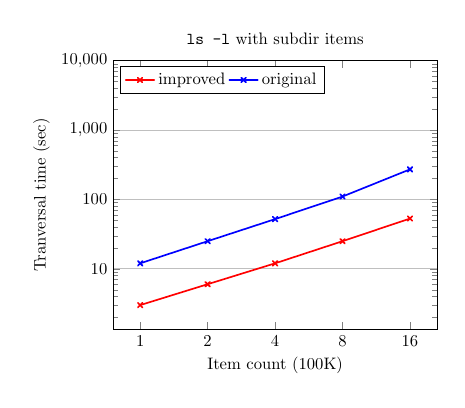
\begin{tikzpicture}[scale=0.6]
            \begin{loglogaxis}[
                xlabel={Item count (100K)},
                log basis x=2,
                xticklabel=\pgfmathparse{2^\tick}\pgfmathprintnumber{\pgfmathresult},
                ylabel={Tranversal time (sec)},
                yticklabel=\pgfmathparse{10^\tick}\pgfmathprintnumber{\pgfmathresult},
                log basis y=10,
                legend style={at={(0.02,0.98)},anchor=north west,cells={anchor=west}},
                legend columns=3,
                title={\texttt{ls -l} with subdir items},
                ymajorgrids,
                ymin=0,ymax=10000,
                ]
                %\axispath\draw
                        %(7.49165,-10.02171)
                    %|-  (8.31801,-11.32467)
                    %node[near start,left] {$\frac{dy}{dx} = -1.58$};

                \addplot[graph,color=red] plot coordinates {
                    (1, 3)
                    (2, 6)
                    (4, 12)
                    (8, 25)
                    (16, 53)
                };
                %
                \addlegendentry{improved}

                \addplot[graph,color=blue] plot coordinates {
                    (1, 12)
                    (2, 25)
                    (4, 52)
                    (8, 110)
                    (16, 271)
                };
                \addlegendentry{original}
            \end{loglogaxis}
        \end{tikzpicture}
    }\makebox[0.5\textwidth][c] {
        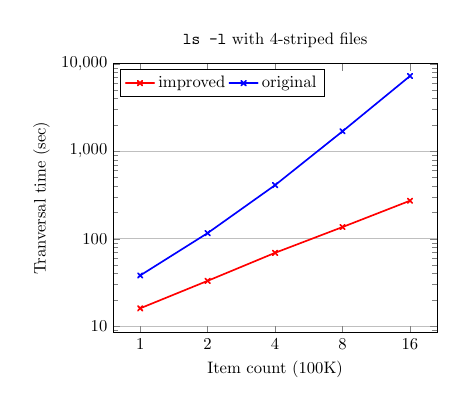
\begin{tikzpicture}[scale=0.6]
            \begin{loglogaxis}[
                xlabel={Item count (100K)},
                log basis x=2,
                xticklabel=\pgfmathparse{2^\tick}\pgfmathprintnumber{\pgfmathresult},
                ylabel={Tranversal time (sec)},
                yticklabel=\pgfmathparse{10^\tick}\pgfmathprintnumber{\pgfmathresult},
                log basis y=10,
                legend style={at={(0.02,0.98)},anchor=north west,cells={anchor=west}},
                legend columns=3,
                title={\texttt{ls -l} with 4-striped files},
                ymajorgrids,
                ymin=0,ymax=10000,
                ]
                %\axispath\draw
                        %(7.49165,-10.02171)
                    %|-  (8.31801,-11.32467)
                    %node[near start,left] {$\frac{dy}{dx} = -1.58$};

                \addplot[graph,color=red] plot coordinates {
                    (1, 16)
                    (2, 33)
                    (4, 69)
                    (8, 136)
                    (16, 272)
                };
                \addlegendentry{improved}

                \addplot[graph,color=blue] plot coordinates {
                    (1, 38)
                    (2, 116)
                    (4, 410)
                    (8, 1692)
                    (16, 7248)
                };
                \addlegendentry{original}
            \end{loglogaxis}
        \end{tikzpicture}
    }

    \vspace{1cm}
    \hfill{\scriptsize\emph{graph data from \cite{metadata-scaling}}}
\end{frame}

\againframe<2>{statdir}

\begin{frame}{SSDs as MDT}
    \begin{itemize}
        \item Metadata often bottleneck
        \item SSDs have higher throughput
        \item SSDs achieve way more IOPS (important for metadata)
        \item only small capacity required (expensiveness!)
    \end{itemize}

    \pause
    Following Graphs:
    \begin{itemize}
        \item plot metadata access (create, stat, unlink)
        \item 8 processes per client-node
        \item HDD/SSD/RAM
        \item shared / per-process directory
        \item ldiskfs / ZFS (Orion-Lustre branch)
        \item data from \cite{mds-eval}
    \end{itemize}
\end{frame}

\newcommand{\ssd}[2]{
    \begin{frame}{SSDs as MDT}
        \scriptsize
        \center
        \begin{tikzpicture}
            \begin{semilogxaxis}[
                xlabel={Client nodes},
                log basis x=2,
                ylabel={#1 per second},
                legend style={font=\tiny,at={(0.02,0.98)},anchor=north west,cells={anchor=west}},
                legend columns=3,
                scaled ticks=false,
                ymajorgrids,
                %xticklabel=\pgfmathparse{2^\tick}\pgfmathprintnumber{\pgfmathresult},
                xtick={0.5,1,2,4,8,16},
                xticklabels={Single Node,1,2,4,8,16},
                width=\textwidth,
                height=7.5cm,
                ]
                %\axispath\draw
                        %(7.49165,-10.02171)
                    %|-  (8.31801,-11.32467)
                    %node[near start,left] {$\frac{dy}{dx} = -1.58$};
                \addplot[graph,unbounded coords=jump,color=red]    table [y index=1] {data/#2.csv}; \addlegendentry{ldiskfs-HDD}
                \addplot[graph,unbounded coords=jump,color=Dandelion] table [y index=2] {data/#2.csv}; \addlegendentry{ldiskfs-SSD}
                \addplot[graph,unbounded coords=jump,color=green]  table [y index=3] {data/#2.csv}; \addlegendentry{ldiskfs-RAM}
                \addplot[graph,unbounded coords=jump,color=purple] table [y index=5] {data/#2.csv}; \addlegendentry{ldiskfs-SSD-SD}
                \addplot[graph,unbounded coords=jump,color=blue]   table [y index=6] {data/#2.csv}; \addlegendentry{ZFS-SSD}
            \end{semilogxaxis}
        \end{tikzpicture}
    \end{frame}
}

\ssd{Creates}{ssd-create}
\ssd{Stats}{ssd-stat}
\ssd{Unlinks}{ssd-unlink}

\subsection{Scalability}
\begin{frame}{Scalability}
    \begin{itemize}
        \item Lustre distributes bandwidth evenly over OSS (striping)
        \item different network types simultaneously (InfiniBand, TCP: GigE)
        \item more OSS can always be added (for more bandwidth and/or capacity)
    \end{itemize}
    \vspace{1cm}
    \pause
    \begin{itemize}
        \item still current bottleneck: MDS
        \item \dots not much data on 2.4 available yet
        \item ZFS improvements required
    \end{itemize}
\end{frame}
